\documentclass{article}
\usepackage{graphicx} % 添加 graphicx 包
\usepackage{amsmath} % 添加 amsmath 包以支持数学公式
\usepackage{geometry} % 添加 geometry 包以调整页面布局
\usepackage{CJKutf8}
\usepackage{setspace} % 添加 setspace 包以调整行间距
\usepackage{hyperref}  % 使目录可以点击跳转
\hypersetup{
    pdfborder={0 0 0}
}
\setcounter{tocdepth}{2}
\geometry{a4paper, margin=1in}

\numberwithin{equation}{section}

\begin{document}
\begin{CJK}{UTF8}{gbsn}
\begin{titlepage}
    \centering
    \vspace*{2cm}
    {\Huge \textbf{Lecture Notes on CS231N}}\\[1.5cm]
    {\Large Yiwei Chen}\\[0.5cm]
    \vfill
    
\includegraphics[width=0.4\textwidth]{images/school_badge.png}\\[1cm] % 确保路径正确
    {\large Zhejiang University}\\[1cm]
    {\large Starting from March 26, 2025}\\[0.5cm]
    {\large Last updated: April 22, 2025}
\end{titlepage}

\onehalfspacing % 设置行间距为 1.5 倍

\tableofcontents % 生成目录
\newpage

\section*{Lecture 1: History of CV and Introduction to CNNs}
\addcontentsline{toc}{section}{Lecture 1: History of CV and Introduction to CNNs}
\setcounter{section}{1}
\setcounter{subsection}{0}
\setcounter{equation}{0}
\begin{itemize}
    \item \textbf{ImageNet:} Annual competition for image classification, started in 2010.
    \item \textbf{Convolutional Neural Networks (CNNs):} Introduced by Yann LeCun in 1998, CNNs are a type of neural network designed for processing structured grid data, such as images. CNNs show great performance in image classification tasks.
\end{itemize}

\newpage

\section*{Lecture 2: Image Classification Pipeline}
\addcontentsline{toc}{section}{Lecture 2: Image Classification Pipeline}
\setcounter{section}{2}
\setcounter{equation}{0}
\subsection{Goal and Attempts}
    \begin{enumerate}
        \item \textbf{Goal:}\par
        The task in Image Classification is to predict a single label (or a distribution over labels as shown here to indicate our confidence) for a given image. Images are 3-dimensional arrays of integers from 0 to 255, of size Width x Height x 3. The 3 represents the three color channels Red, Green, Blue.\par
        \item \textbf{Attempts:}
        \begin{itemize}
            \item Find edges, then corners: does not work well.
            \item Use large datasets with labels.
        \end{itemize}
    \end{enumerate}


\subsection{Classifiers:}
    \begin{enumerate}
        \item \textbf{K-Nearest Neighbors (KNN):}
        \begin{itemize}
            \item \textit{Description:} When \(K = 1\), Find the closest image in the dataset to the input image (Nearest Neighbors (NN)).
            \item \textit{Distance metric:}
            \begin{enumerate} 
                \item L1(Mahanttan) Distance: a squared distance metric.
                \begin{equation}
                    d(x,y) = \sum_i |x_i - y_i|
                \end{equation}
        
                \item L2(Euclidean) Distance: a squared distance metric.
                \begin{equation}
                    d(x,y) = \sqrt{\sum_i (x_i - y_i)^2}
                \end{equation}
            \end{enumerate}
            \textit{Rotating the coordinate system changes the L1 distance but not the L2 distance.}
            
            \item \textit{Performance:}\par
            Training time: \(O(1)\), as there is nothing to do.\par
            Prediction time: \(O(N)\), which is inefficient.
        
            \item K-Nearest Neighbors (KNN):\par
            \textit{Description:} \par
            When \(K = 1\), the classifier is too sensitive to noise.\par
            Instead of copying the label of the closest image, take the majority vote of the \(K\) closest images.
            \item \textit{hyperparameters}(超参数):\par
            Choices about the model that are not learned from the data, e.g., \(K\) in KNN.\par
            \textit{To set hyperparameters:}\par
            \begin{itemize}
                \item Never use the test set to set hyperparameters.\par
                \item Splitting data into train and test is not enough.\par
                \item \textbf{The better idea:} Splitting the training set into training set, validation set, and test set.\par
                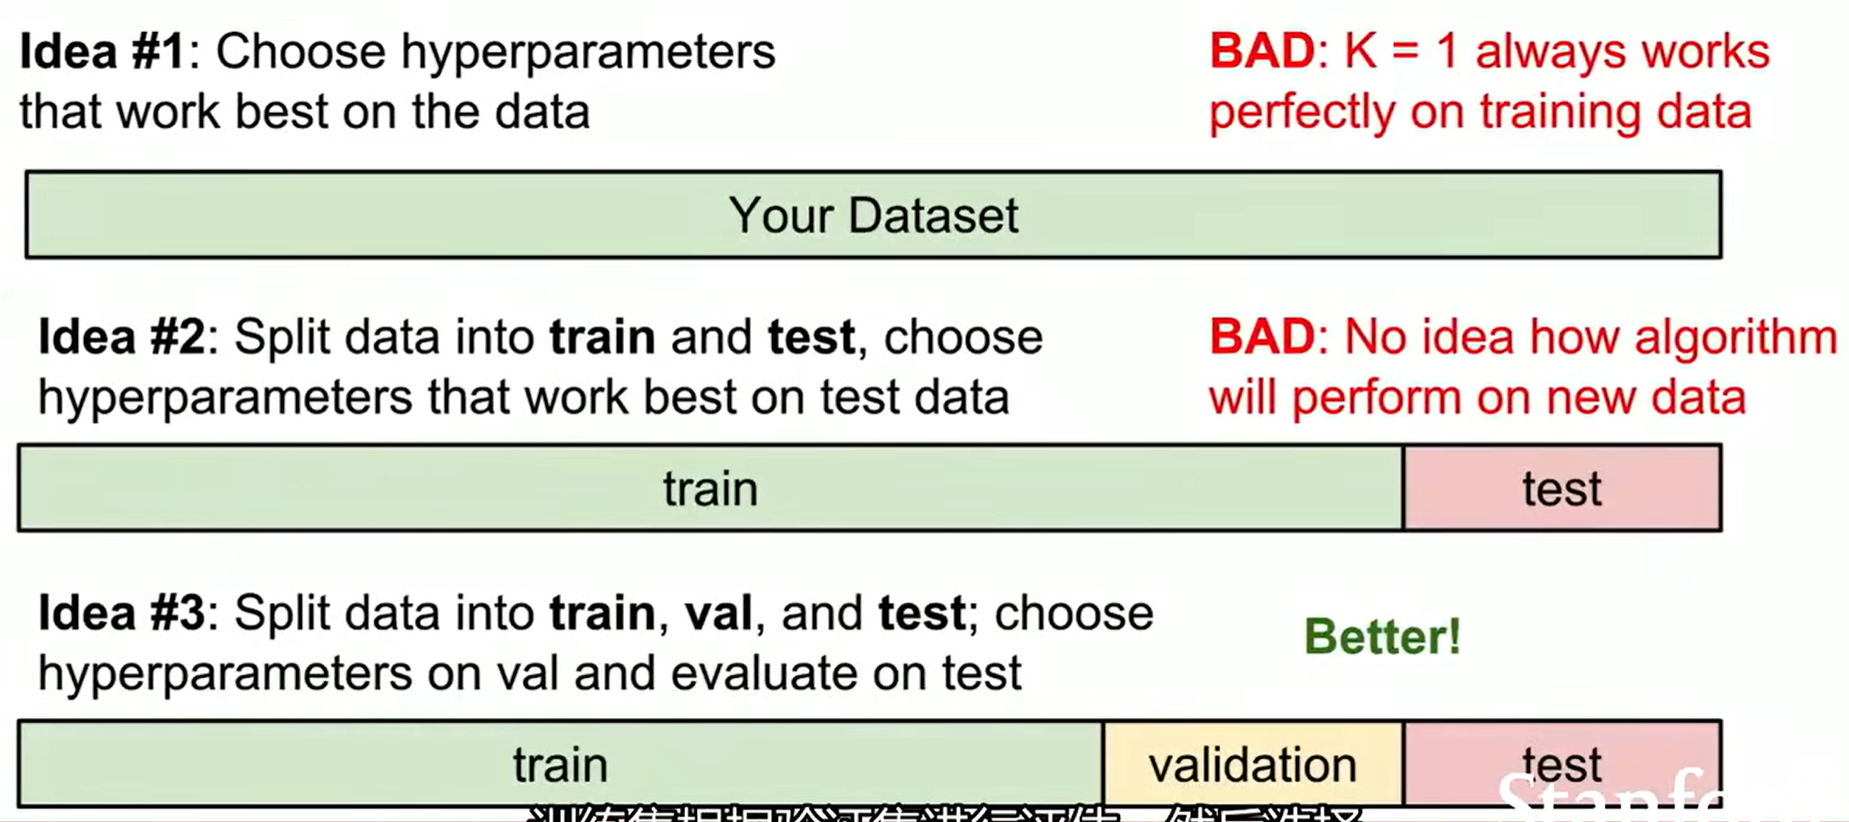
\includegraphics[width=0.8\textwidth]{images/Lecture2/ideas_for_hyperparameter.png}
                \item \textbf{The common idea:} Cross-validation(交叉验证).\par
                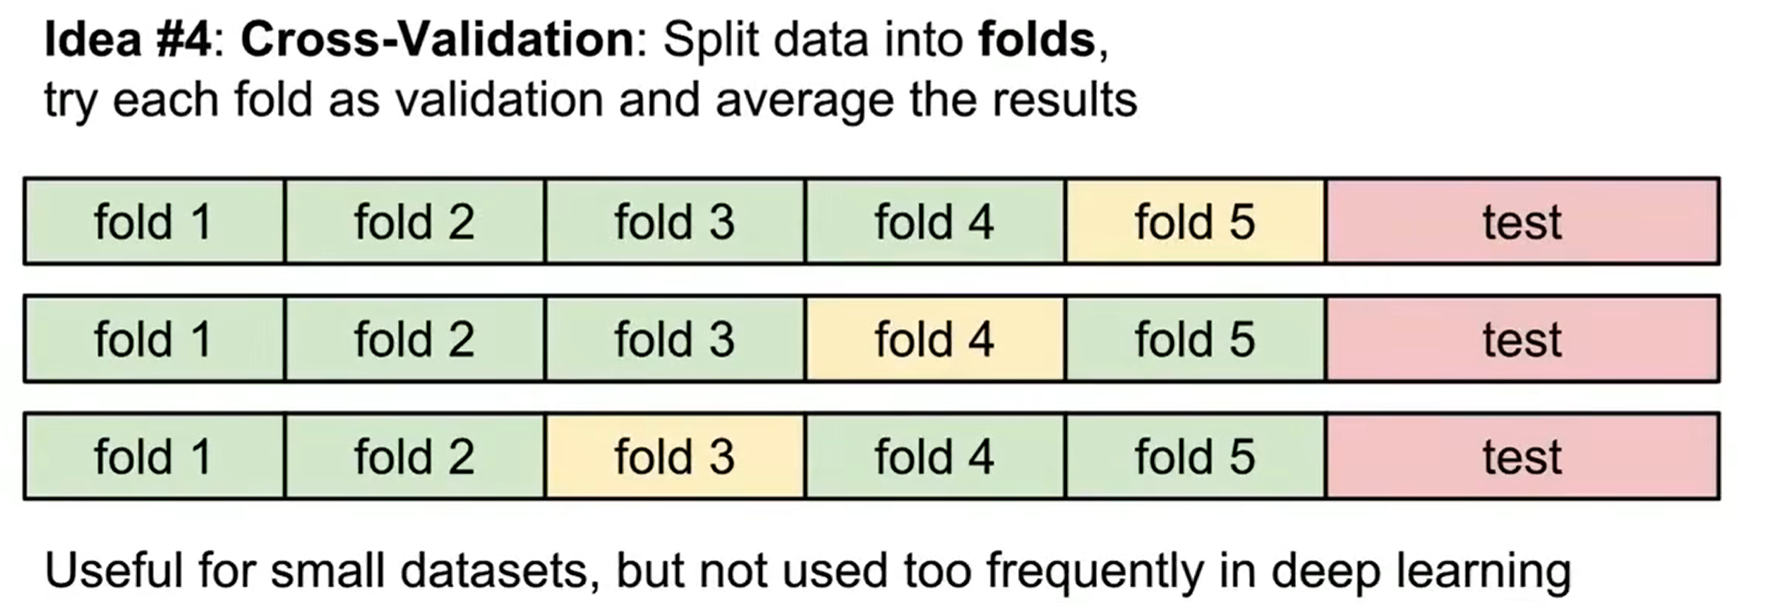
\includegraphics[width=0.8\textwidth]{images/Lecture2/cross_validation.png}
            \end{itemize}

            \item \textit{Pros and Cons:}\par
            Actually, KNN on image is never used:\par
            - Very slow at test time.\par
            - Distance-metrics on pixels are not informative.\par
            - Curse of dimensionality: as the number of dimensions increases, the distance between points becomes less meaningful.\par
        \end{itemize}

        \item \textbf{Linear Classifier:}
        \begin{itemize}
            \item \textit{Description:} A linear classifier makes its predictions based on a linear predictor function combining a set of weights with the feature vector.\par
            \begin{equation}
                f(x, W) = Wx + b
            \end{equation}
            where \(x\) is the input image and \(w\) is the weight vector, \(b\) is the bias term.\par
            And it is important to center the data before applying the linear classifier, namely image data preprocessing.\par
            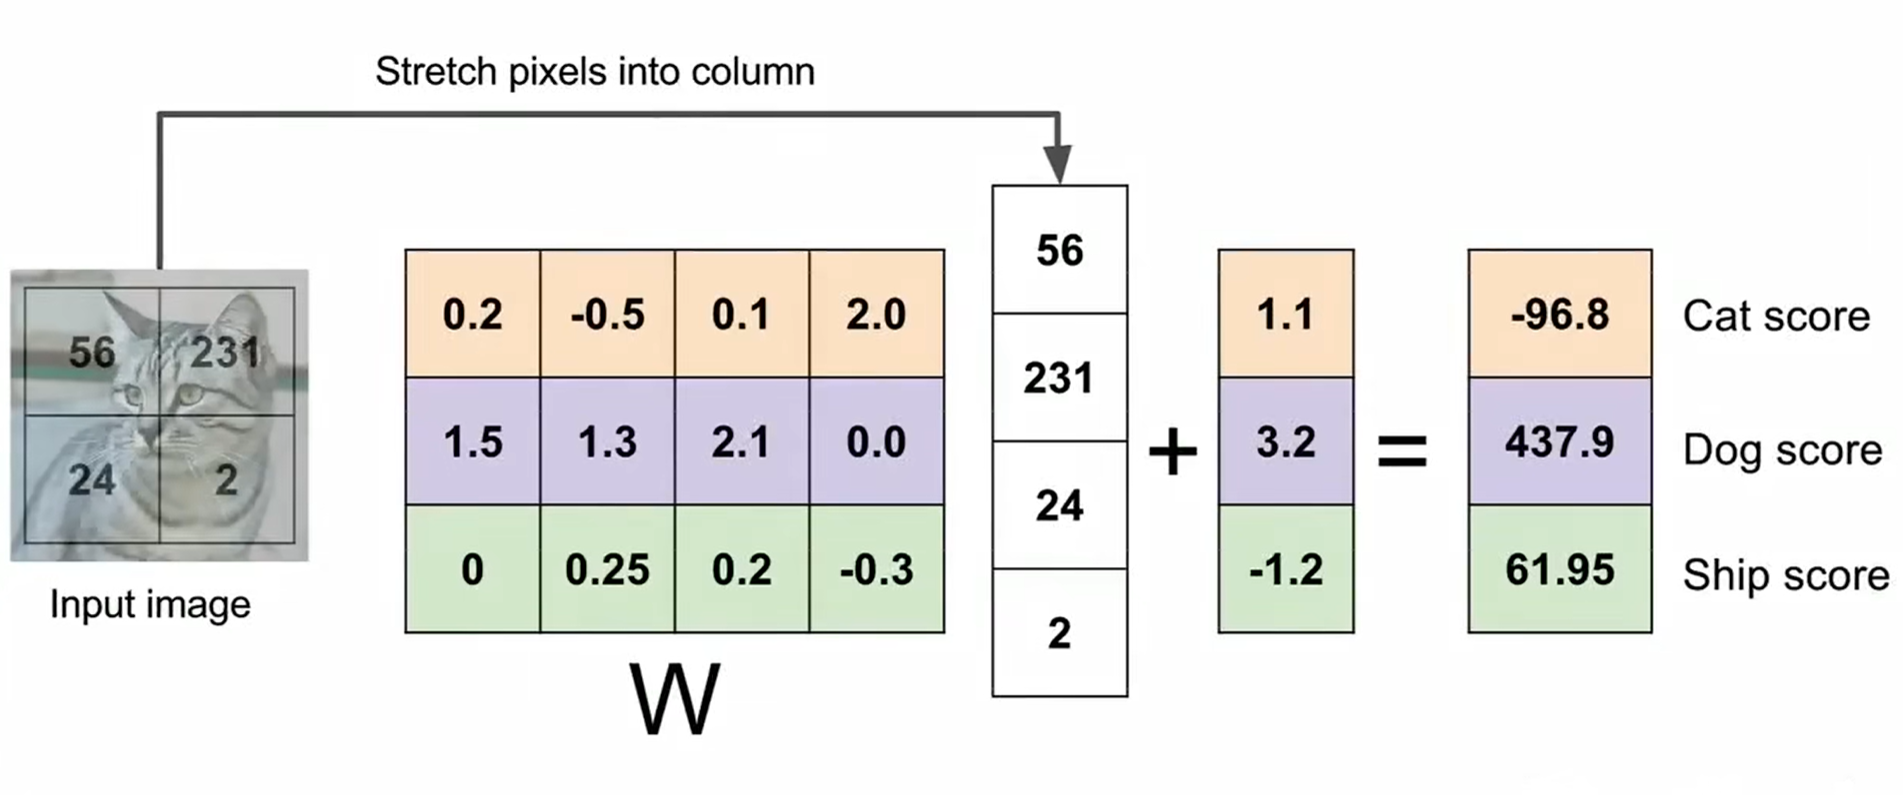
\includegraphics[width=0.8\textwidth]{images/Lecture2/linear_classifier_example.png}
            \item \textit{Hard cases:}\par
            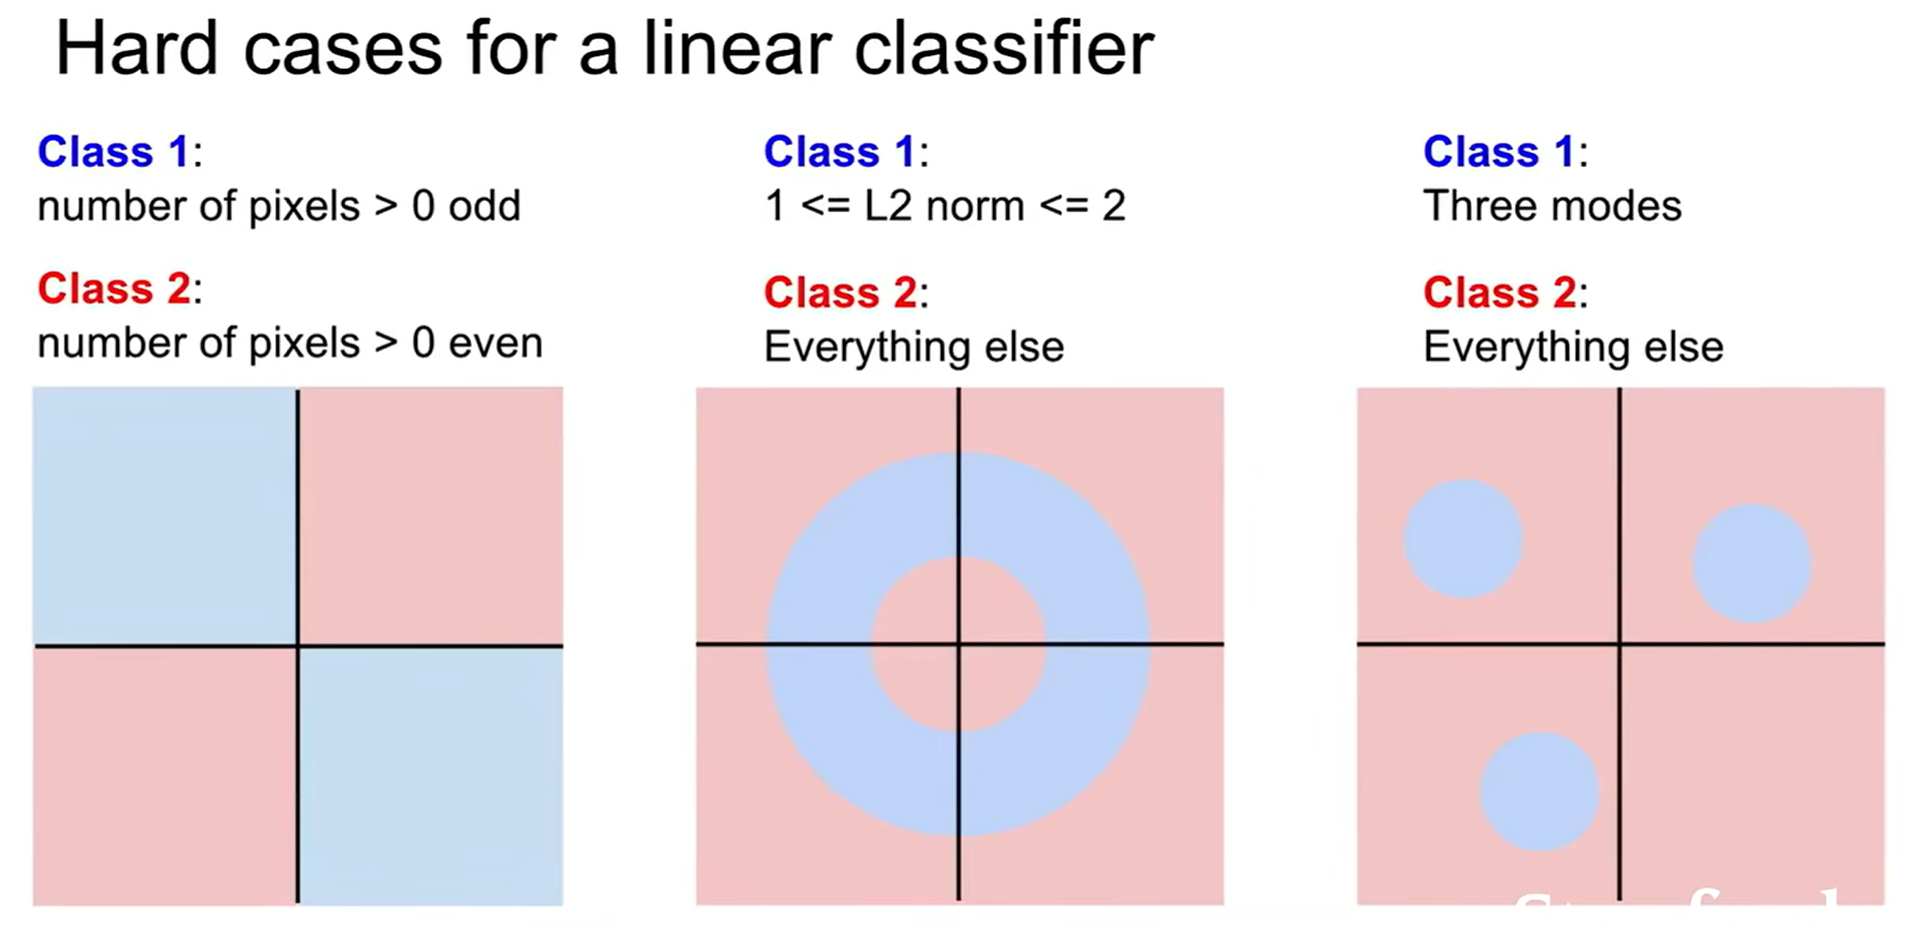
\includegraphics[width=0.8\textwidth]{images/Lecture2/hard_cases_for_linear_classifier.png}
        \end{itemize}
    \end{enumerate}



\newpage
\section*{Lecture 3: Loss Functions and Optimization}
\addcontentsline{toc}{section}{Lecture 3: Loss Functions and Optimization}
\setcounter{section}{3}
\setcounter{subsection}{0}
\setcounter{equation}{0}

\subsection{Loss Functions}
\begin{enumerate}
    \item \textbf{Multiple SVM loss:}\par
    \begin{equation*}
        L_i = \sum_{j \neq y_i} \begin{cases}
            0 & \text{if } s_{y_i} \geq s_j + 1 \\
            s_{y_i} - s_j + 1 & \text{otherwise } 
        \end{cases}
    \end{equation*}
    
    \begin{equation}\tag{SVM-Loss}
        L_i = \sum_{j \neq y_i} \max(0, s_j - s_{y_i} + 1) = \sum_{j \neq y_i} \max(0, w^T_j x_j - w^T_{y_i} x_{y_i} + 1)
    \end{equation}
    where \(y_i\) is the label for class \(i\), \(s = f(x_i, W)\) is the score for class \(i\), where wj
    is the j-th row of W \textbf{reshaped as a column}.\par

    And this kind of loss function is called \textbf{Hinge Loss}.\par
    \begin{figure}[h]
        \centering
        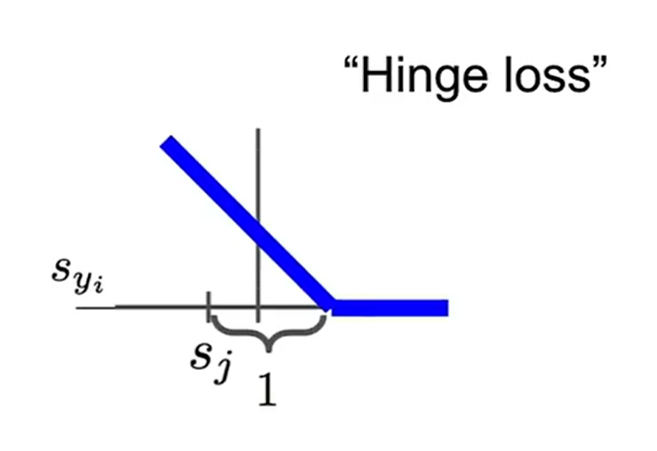
\includegraphics[width=0.6\textwidth]{images/Lecture3/Hinge_loss.png}
    \end{figure}

    \begin{equation}
        L = \frac{1}{N} \sum_{i=1}^{N} L_i
    \end{equation}

    For the first training, the W is randomly initialized, so the loss is close to C - 1, where C is the number of classes, which can be used to check the correctness of the implementation.\par

    \item \textbf{regularization:}\par
    Furthermore, we can add a regularization term to the loss function to prevent overfitting:
    \begin{equation}
        L = \frac{1}{N} \sum_{i=1}^{N} L_i + \lambda R(W) = \frac{1}{N} \sum_{i=1}^{N} \sum_{j \neq y_i} \max(0, f(x_i, W)_j - f(x_i, W)_{y_i} + \Delta) + \lambda R(W)
    \end{equation}
    Here \(\Delta\) actually does not matter. It turns out that this hyperparameter can safely be set to \(\Delta=1.0\) in all cases.\par
    The hyperparameters \(\Delta\) and \(\lambda\) seem like two different hyperparameters, but in fact they both control the same tradeoff: The tradeoff between the data loss and the regularization loss in the objective.\par
    Therefore, the exact value of the margin between the scores is in some sense meaningless because the weights can shrink or stretch the differences arbitrarily. Hence, the only real tradeoff is how large we allow the weights to grow (through the regularization strength \(\lambda\)).\par
    In common use:
    \begin{itemize}    
        \item \textbf{L2 regularization:} \(R(W) = ||W||^2\)
        \item L1 regularization: \(R(W) = ||W||_1\)
        \item Elastic net: \(R(W) = \beta ||W||^2 + ||W||_1\)
        \item Max norm regularization: might see later
        \item Dropout: might see later
        \item Fansier: Batch normalization, stochastic depth, etc.
    \end{itemize}

    \item \textbf{Softmax Classifier(Multinomial Logistic Regression):}\par
    scores = unormalized log probabilities of the classes.\par
    \begin{equation}
        P(y_i | x_i) = \frac{e^{s_{y_i}}}{\sum_{j=1}^{C} e^{s_j}} \quad \text{where } C \text{ is the number of classes}
    \end{equation}

    \begin{equation}
        L_i = -\log P(y_i | x_i) = -\log \frac{e^{s_{y_i}}}{\sum_{j=1}^{C} e^{s_j}} = -s_{y_i} + \log \sum_{j=1}^{C} e^{s_j}
    \end{equation}

    For Softmax, even though the right score is much higher than all the other scores, the loss is still not zero, which is different from SVM.\par
    
    Here, it's actually a cross-entropy loss function, which is defined as follows:
    \begin{equation*}\tag {Cross-entropy}
        H(p, q) = -\sum_{x} p(x) \log q(x)
    \end{equation*}
    where \(p\) is the "true" distribution and \(q\) is the predicted distribution.\par
    For Softmax, \(q = e^{s_j} / \sum_{k=1}^{C} e^{s_k}\), and the "true" distribution is a one-hot vector(p = [0,...,1,...,0] contains a single 1 at the \(y_i\)-th position).\par
\end{enumerate}

\subsection{Optimization:}
    Strategy: follow the slope

    So first we need to compute the gradient of the loss function with respect to the weights \(W\).\par
    The method of finite differences(\((f(W+h) - f(W)) / h\)) is bad because of large amount of computation, dont't use it to train but to \textbf{check the correctness} of the implementation.\par

    \vspace{0.5cm}
    \textbf{step size/learning rate:} a hyperparameter that controls how much to change the model in response to the estimated gradient.\par

    \begin{enumerate}
        \item \textbf{Derivative of the loss function:}\par
        \begin{equation}
        \nabla_W L(W) = \frac{1}{N} \sum_{i=1}^{N} \nabla_W L_i(x_i, y_i, W) + \lambda \nabla_W R(W)
        \end{equation}

        The scores of each class are influenced by the rows of \(W\) corresponding to the classes.\par
        Hence, the gradient of the loss function with respect to the weights \(W\) should focus on the rows.(assuming W is (C * D))\par
        
        \begin{itemize}
            \item \textbf{For Hinge Loss:}\par
            \begin{equation*}
                L_i = \sum_{j \neq y_j} [\max(0, w^T_j x_i - w^T_{y_i} x_i + \Delta)]
            \end{equation*}
            where \(w_j\) is the j-th row of W reshaped as a column.\par
            \
            
            Taking the gradient with respect \(w_{y_i}\)
            \begin{equation}
                \nabla_{w_{y_i}} Li = - (\sum_{j \neq y_j}1(w^T_j x_j - w^T_{y_i} x_{y_i} + \Delta > 0)) x_i
            \end{equation}
            where 1 is the indicator function that is one if the condition inside is true or zero otherwise. 
        
            For the other rows where \(j \neq y_i \) (for every j) the gradient is:
            \begin{equation}
                \nabla_{w_j} Li = 1(w^T_j x_j - w^T_{y_i} x_{y_i} + \Delta > 0)  x_i
            \end{equation}

            \item \textbf{For Softmax Loss:}\par
            \begin{equation*}
                L_i = -\log P(y_i | x_i) = -\log \frac{e^{s_{y_i}}}{\sum_{j=1}^{C} e^{s_j}} = -s_{y_i} + \log \sum_{j=1}^{C} e^{s_j}
            \end{equation*}

            Taking the gradient with respect \(w_{y_i}\)
            \begin{equation}
                \nabla_{w_{y_i}} Li = -x_i + \frac{e^{s_{y_i}}}{\sum_{j=1}^{C} e^{s_j}} x_i = -x_i + P(y_i | x_i) x_i
            \end{equation}
            
            For the other rows where \(j \neq y_i \) (for every j) the gradient is:
            \begin{equation}
                \nabla_{w_j} Li = \frac{e^{s_j}}{\sum_{k=1}^{C} e^{s_k}} x_i = P(j | x_i) x_i
            \end{equation}
        
        \end{itemize}
    
        \item \textbf{Stochastic Gradient Descent(on-line gradient descent):}\par
        Full sum computation is too expensive, so we can use mini-batch(32/64/128) gradient descent.\par
        Every iteration, we randomly sample a mini-batch of \(N\) training examples from the training set, and compute the gradient of the loss function with respect to the weights \(W\) using only this mini-batch.\par
        
        SGD technically refers to using a single example at a time to evaluate the gradient.\par
        However, you will hear people use the term SGD even when referring to mini-batch gradient descent (i.e. mentions of MGD for “Minibatch Gradient Descent”, or BGD for “Batch gradient descent” are rare to see), where it is usually assumed that mini-batches are used.\par
        MGD: using a small batch of examples to evaluate the gradient.\par
        BGD: using the entire training set to evaluate the gradient.\par
    \end{enumerate}

\subsection{Image features:}
    Some times, only using the raw pixel values is not enough, we need to extract some features from the image.\par
    For example:
    \begin{itemize}
        \item color histogram(直方图): a representation of the distribution of colors in an image.
        \item HOG(Histogram of Oriented Gradients): a feature descriptor focusing on the edges and contours of objects in an image.
        \item Bag of Words: a representation of an image as a collection of local features, where each feature is represented by a visual word.
    \end{itemize}



\newpage
\section*{Lecture 4: Backpropagation and Neural Networks}
\addcontentsline{toc}{section}{Lecture 4: Backpropagation and Neural Networks}
\setcounter{section}{4}
\setcounter{subsection}{0}
\setcounter{equation}{0}

\subsection{Backpropagation}
\begin{enumerate}
    \item \textbf{Computation Graph:}\par
    \begin{figure}[h]
        \centering
        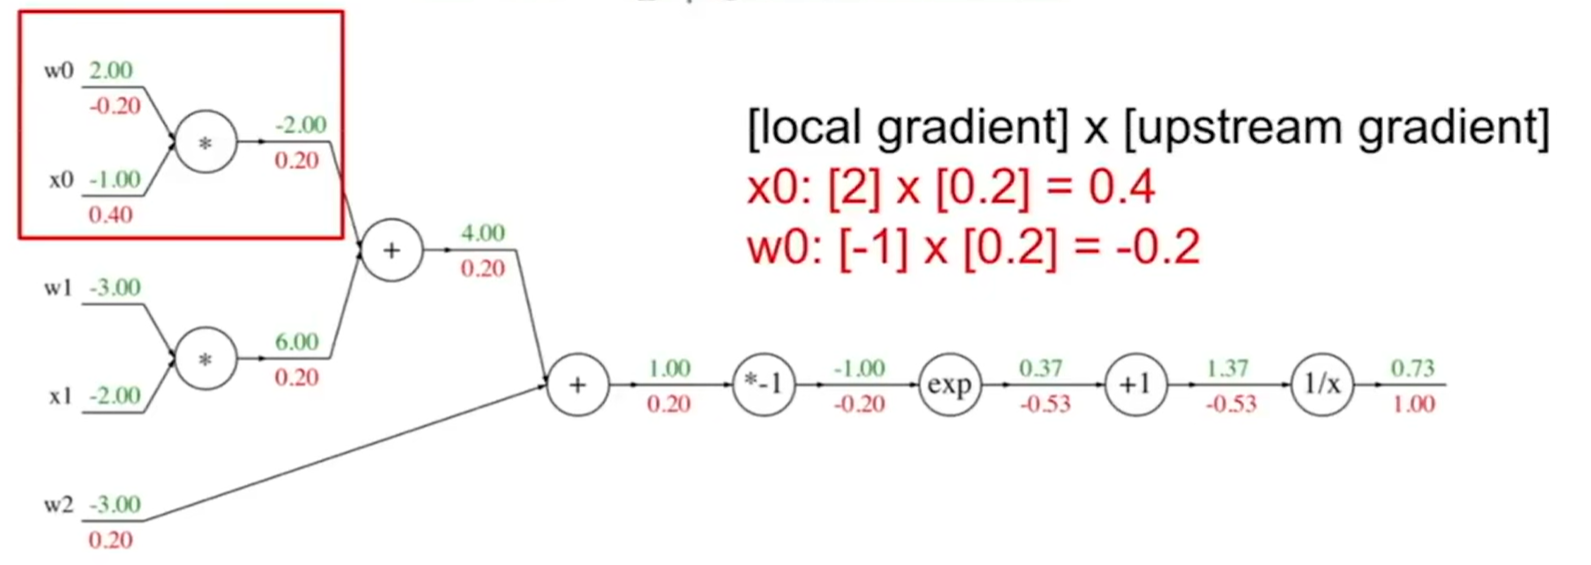
\includegraphics[width=0.8\textwidth]{images/Lecture4/computation_graph.png}
        \caption{Computation Graph Example: \(f(x) = \frac{1}{1 + e^{-(\omega_0 x_0 + \omega_1 x_1 + \omega_2)}}\)}
        \label{fig:computation_graph}
    \end{figure}
    Along the edges of the graph, we do \textbf{forward} computations to get the scores of the classes, and get the output label.\par
    And \textbf{backward} computations to get the gradients of the loss function with respect to the weights \(W\) and the input \(x\).\par


    \item \textbf{Backpropagation}\par

        \textbf{Sigmoid funtion:}
        \begin{equation}
            \sigma(x) = \frac{1}{1 + e^{-x}}
        \end{equation}
        It is a common activation function used in neural networks, especially in the output layer for binary classification tasks.\par
        \begin{figure}[h]
            \centering
            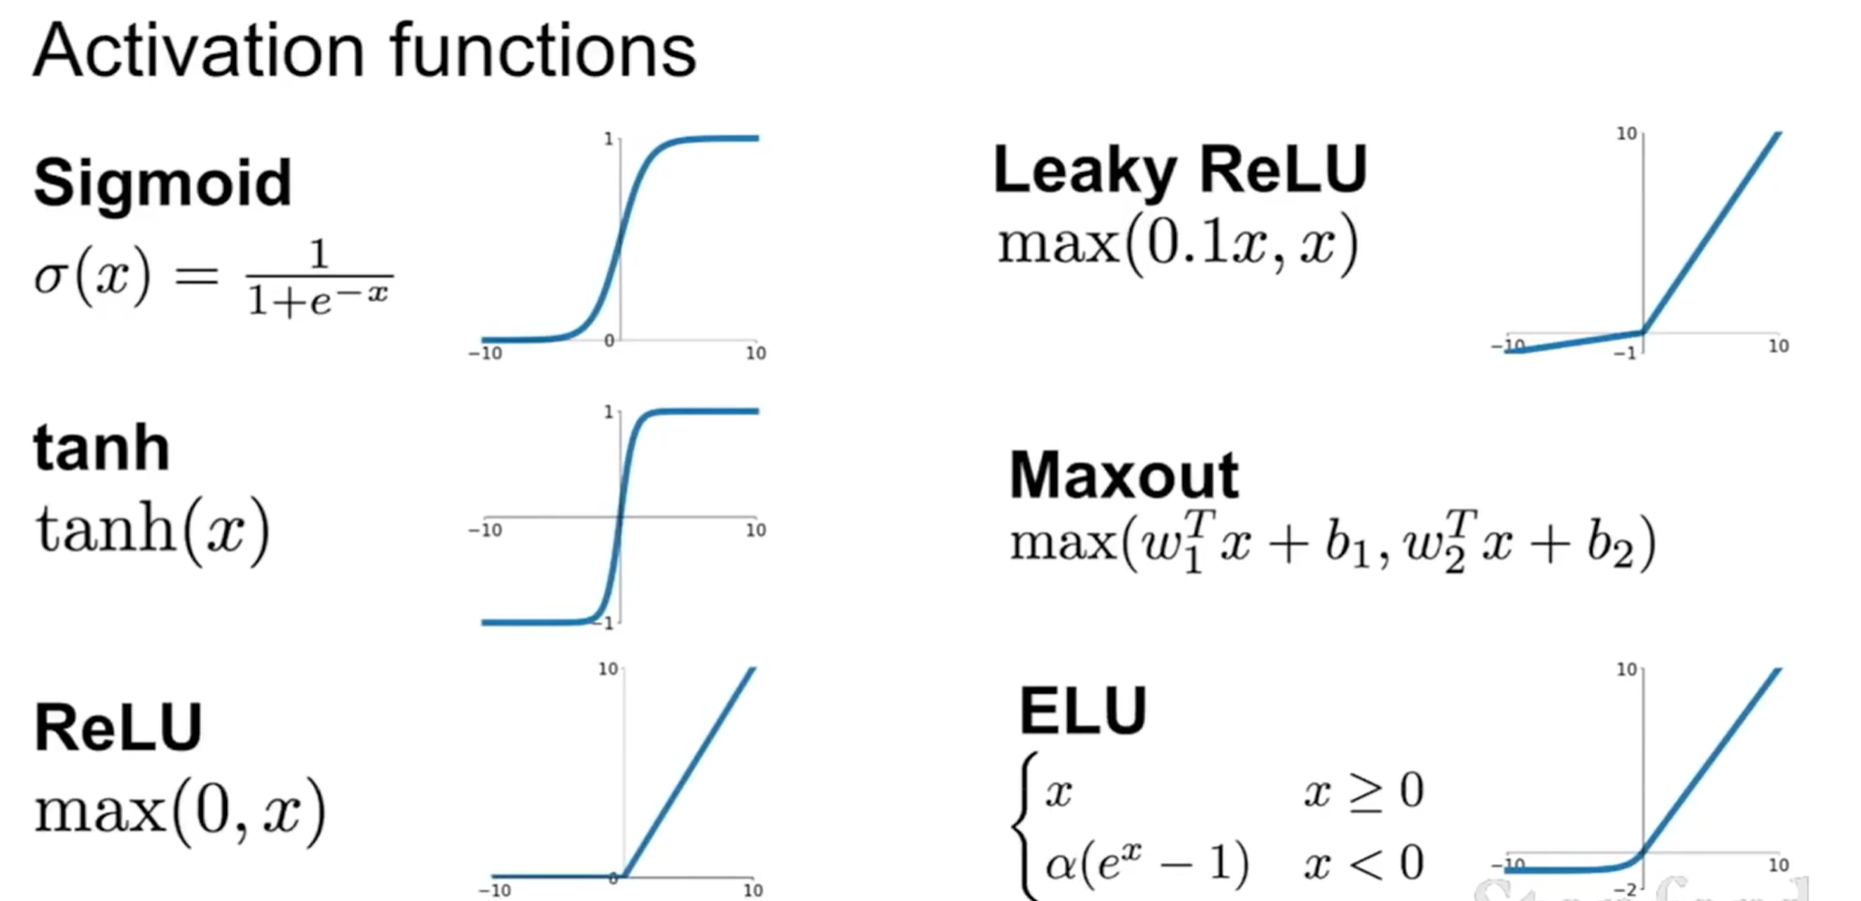
\includegraphics[width=0.8\textwidth]{images/Lecture4/activation_functions.png}
            \caption{Activation Functions}
            \label{fig:activation_functions}
        \end{figure}

        \begin{itemize}
            \item \textbf{Add gate:} gradient distributor\par
            \item \textbf{Max gate:} gradient router\par
            only the maximum value will pass through the gate, and the others will be zero.\par
            \item \textbf{Mul gate:} gradient switcher\par
        \end{itemize}

        Additionally, if the element is a vector, the gradient will be Jacobian matrix with the same shape as the input.\par
        For f(x, W) = Wx + b(x is a batch), the gradient is:
        \begin{equation}
            \nabla_x = dout * W^T ,\quad \nabla_W = x^T * dout ,\quad \nabla_b = \sum dout * 1
        \end{equation}

\end{enumerate}

\newpage
\subsection{Neural Networks:}
    \begin{figure}[h]
        \centering
        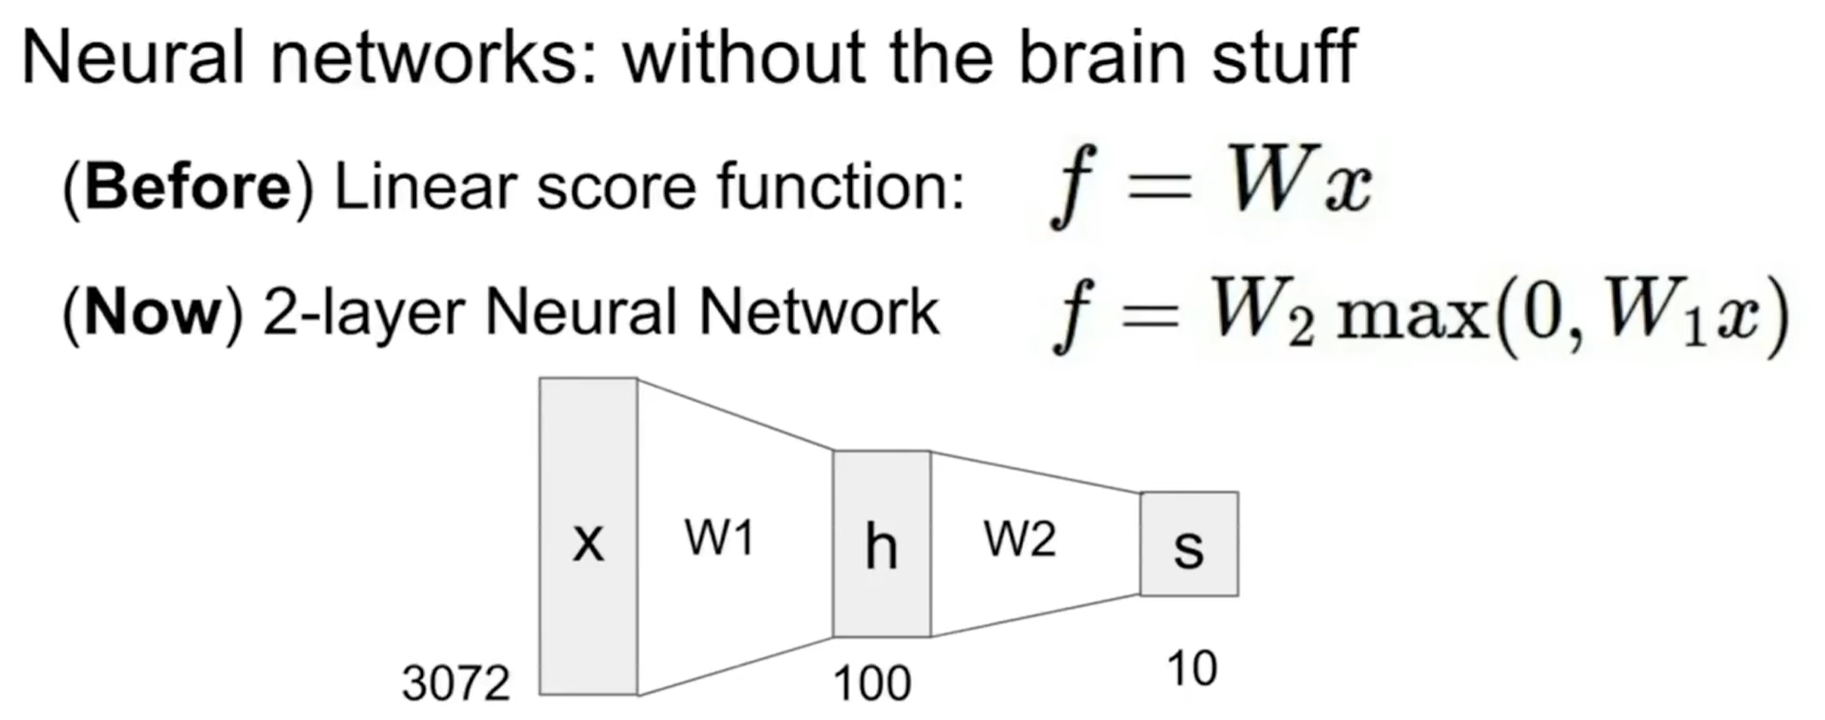
\includegraphics[width=0.8\textwidth]{images/Lecture4/two_layer_neural_network.png}
        \caption{Neural Network Example: \(f(x) = W_2 \max(0, W_1 x)\)}
        \label{fig:neural_network}
    \end{figure}
    Here, \(W_1\) contains the weights for the first layer, which can be thought of as computing the scores of the templates.\par
    And \(W_2\) contains the weights for the second layer, which can be thought of as computing the final scores for the classes by taking a weighted sum of the scores from the first layer.\par

    Below are figures showing the structure of a neural network.\par
    \begin{figure}[h]
        \centering
        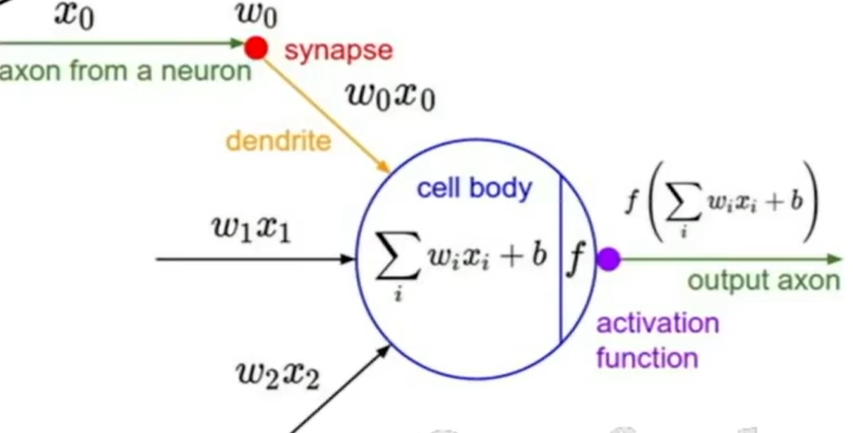
\includegraphics[width=0.6\textwidth]{images/Lecture4/neural_like.png}
        \caption{Neuron-like structure}
        \label{fig:neural_like}
    \end{figure}

    \begin{figure}[h]
        \centering
        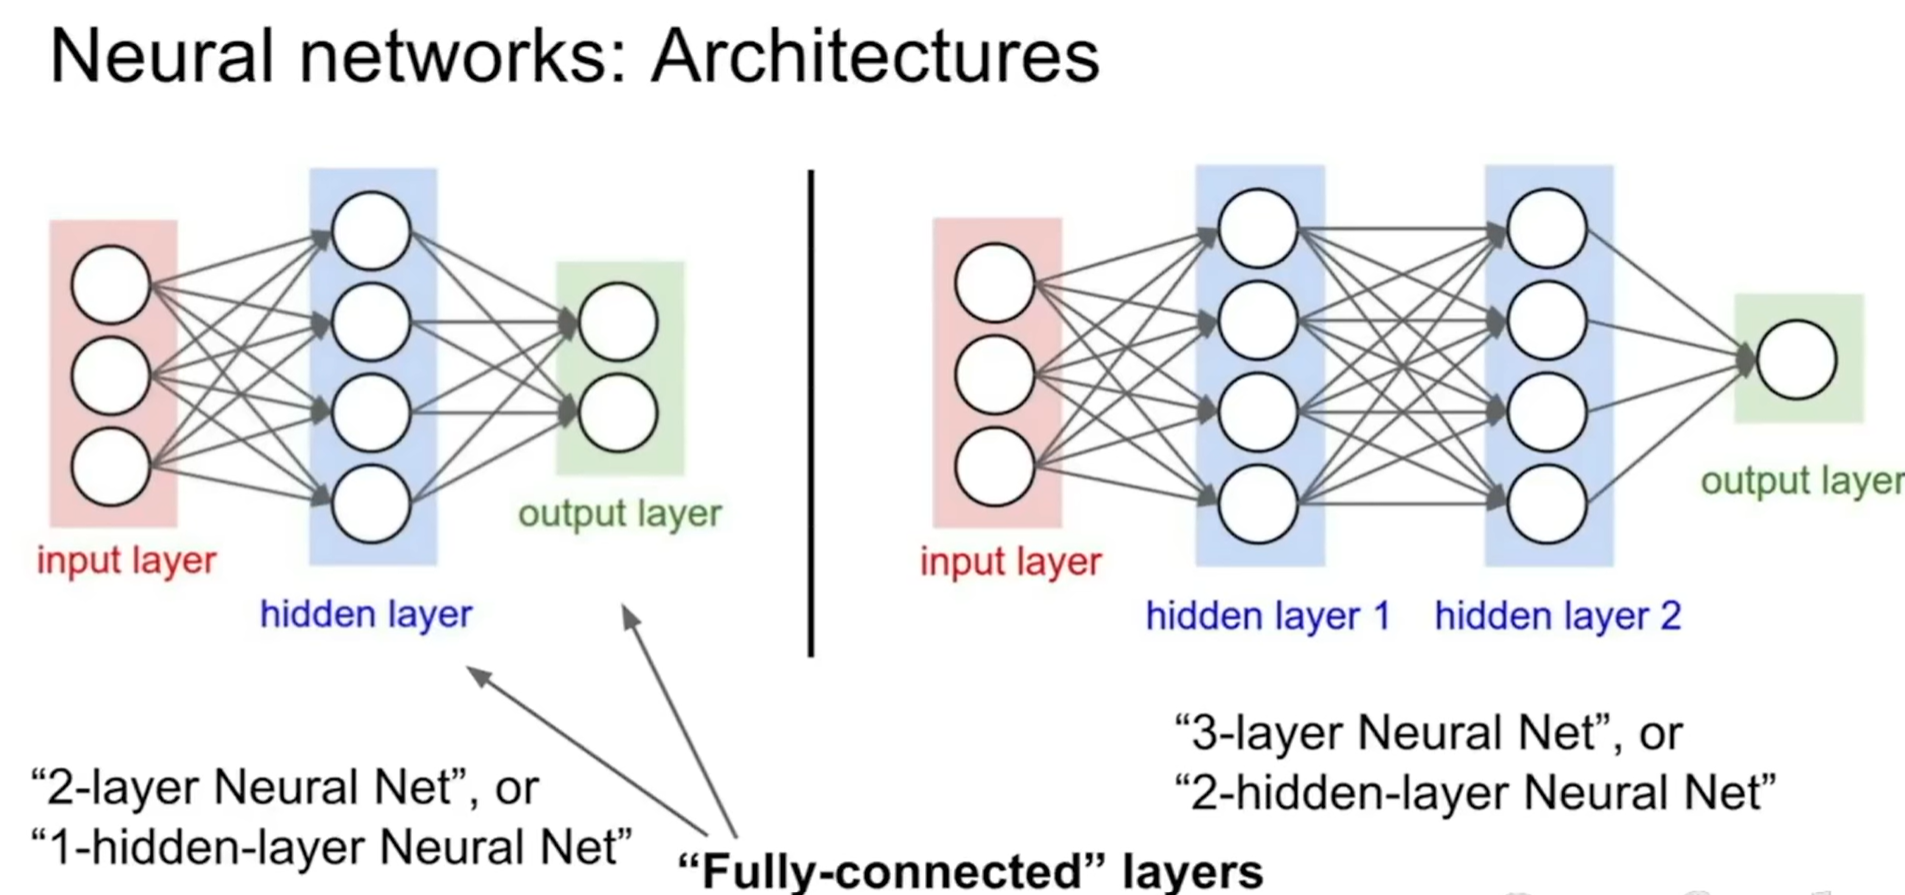
\includegraphics[width=0.6\textwidth]{images/Lecture4/neural_network_arch.png}
        \caption{Neural Network Architecture}
        \label{fig:neural_network_arch}
    \end{figure}

\newpage
\section*{Lecture 5: Convolutional Neural Networks}
\addcontentsline{toc}{section}{Lecture 5: Convolutional Neural Networks}
\setcounter{section}{5}
\setcounter{subsection}{0}
\setcounter{equation}{0}

\subsection{Convolution Layer}
Instead of stretching the input image into a long vector, now preserve the spatial structure.\par
\begin{itemize}
    \item \textbf{Filter:} Filters always extend the full \textbf{depth} of the input volume.\par
    Convolve(slide) over all spatial locations.
    Each filter is kind of looking for a specific feature in the image, so usually we have many filters in a convolutional layer.\par

    \begin{figure}[h]
        \centering
        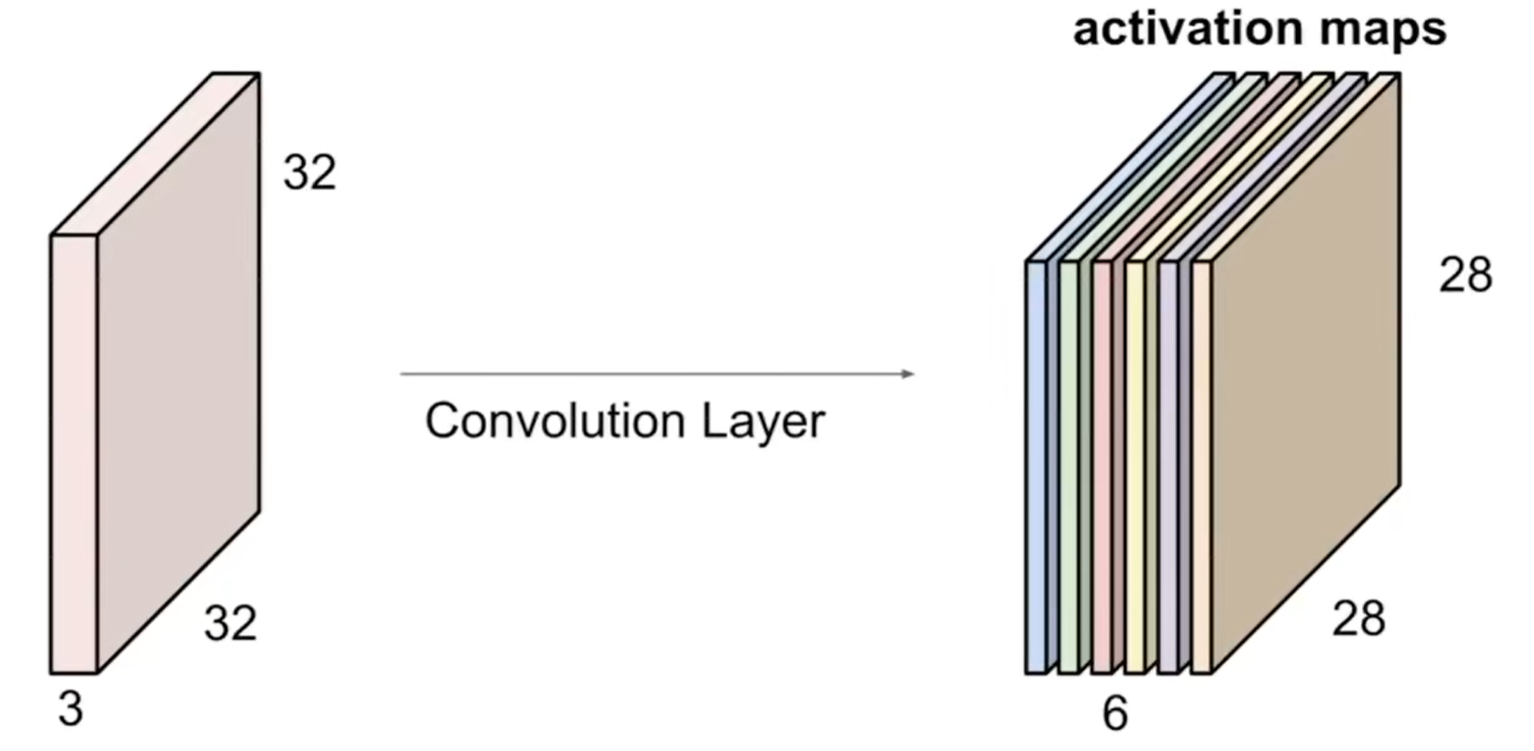
\includegraphics[width=0.8\textwidth]{images/Lecture5/Convolution_layer.png}
        \caption{Convolution Operation}
        \label{fig:convolution}
    \end{figure}

    \item \textbf{Convolution:}\par
    In mathematical terms, the convolution operation is defined as:
    \begin{equation}
        f[x, y] * g[x, y] = \sum_{n_1=-\infty}^{\infty} \sum_{n_2=-\infty}^{\infty} f[n1, n2] * g[x-n1, y-n2]
    \end{equation}
    which means that the filter is flipped both horizontally and vertically before being applied to the image.\par

    What we commonly do is a cross-correlation(互相关) operation, without flipping the filter, but we call it convolution.\par
    


\end{itemize}

\end{CJK}
\end{document}




